\documentclass[a4paper,11pt]{article}
\usepackage[osf]{mathpazo}
\usepackage{ms}
\usepackage[]{natbib}
\raggedright

\newcommand{\smurl}[1]{{\footnotesize\url{#1}}}
\usepackage{graphicx}

\title{Toward dynamic models of combat or lack thereof in animal mating}
\author{
* John Wilshire$^1$, Will Cornwell$^1$ , Daniel Falster$^2$, Michael Kasumovic$^1$, \\
Daniel Noble$^1$,$^1$ Loic Thibaut$^1$}
\affiliation{
*final list and order undecided\\
$^1$ University of NSW\\
$^2$ Macquarie University\\
}
\date{}

\bibliographystyle{mee}

\usepackage[title,titletoc,toc]{appendix}

\mstype{Research Article}
\runninghead{A new framework for fighting}
\keywords{}

\begin{document}
\mstitlepage
\noindent
% \doublespacing
% \linenumbers

\section{Summary}
The diversity of animal mating systems is astounding. In some of these
systems, very costly combat behaviour -- among males, among females, or
both -- is a feature of the mating process.  In other systems, resources
are divided among individuals in an entirely pacific process.  Can we
understand why? Animal combat strategies likely emerge from trade-offs
in investment in growth, mate seeking, and information gathering.
Willingness to engage in combat is a trait that evolves based on the
fitness landscape, which itself changes depending on both the
environment and the strategies of other individuals.  Using recently
developed methods for modelling dynamic fitness landscapes, we examine:
(1) why combat behaviours arise, (2) under what conditions combat
behaviours are evolutionarily stable, and (3) when different combat
strategies co-exist.  We hypothesize that the reliability and
"public-ness" of information is an important feature driving combat or
lack thereof in many animal systems.

\section{Introduction}

Evolution of animal personalities: \citep{Wolf-2007,Wolf-2012} show can have
coexistence of risky, explorative strategies and risk-averse strategies.

Animal personalities linked to other life history traits: \citep{Biro-2008}

Individual-based models of natural selection: \citep{MGonigle-2012}


\section{Methods}

% Verbal description of model

We consider a population of males competing for mates. The population is one with non-overlapping generations, and within each generation there is a predefined annual cycle. In spring, up to $K$individuals hatch from eggs, grow throughout spring and summer to increase size, and then within a short period, the entire population mates, females lay eggs and everyone dies. The short duration of mating period is such that each male and female only mates once. The population then re-establishes from eggs the following spring.

The reproductive success of males in the population is determined via their ability to compete for and hold $N$ nests. Nests differ in quality (potential number of offspring per nest per year). The male population is divided into two groups: immature and mature males. Immature males devote all their efforts towards feeding, increasing their size. Males mature with a probability defined by their size and a maturation trait. Once they enter the mature population, males stop feeding and focus solely on obtaining nests. Nests can be vacant or occupied and males are either ``searching'' or ``occupying'' a nest. Males differ in the rate at which they search, and thus the rate at which they encounter nests. Empty nests can be immediately occupied with no additional cost. Filled nests can only be obtained by entering into and winning a contest. Once occupied, males can choose to occupy a nest or continue searching. At the end of each season, each male has a fitness defined by the reproductive value of the nest it holds, $R_i$.

\subsection{Habitat}

Denote $N$ to be the total number of available nests, $R_i$ to be the reproductive value of nest $i$ (number of offspring per nest per year), $\bar{R}$ to be the average reproductive value of all nests (number of offspring per nest per year), and $p(R)$ to be the probability density distribution of nest quality with respect to $R$. The distribution of nest qualities is then set according to the distribution
\begin{equation} \label{eq:pdf_R}
Pr(R_i = x) =\bar{R} \, p(R).
\end{equation}
The total number of male offspring produced in each generation is then
\begin{equation} \label{eq:pdf_R}
K = \bar{R} N.
\end{equation}

\subsection{Immature phase}

Within the immature phase, we assume males grow with rate
\begin{equation} \label{eq:growth}
\frac{{\rm d} m}{{\rm d} t} = a \, m^ b
\end{equation}
where $a$ is mass-based rate of growth. Integrating eq. \ref{eq:growth}, the size of individuals at time $t$, having started growing at time $0$ is given by
\begin{equation} \label{eq:growth}
m(t) = \left(m(0)^{1-b} + t a(1-b)\right)^{\frac1{1-b}},
\end{equation}
while the time $\tau$ taken for a male to grow from $m(0) \rightarrow m$ is then
\begin{equation} \label{eq:tau}
\tau(m_0, m) = \frac1{a(1-b)}\left(m ^{1-b} - m_0 ^{1-b}\right).
\end{equation}

If we assume a constant mortality rate $k_i$ during the immature phase, the probability of males surviving to time $t$ is given by
\begin{equation} \label{eq:surv_immature}
S(t) = \exp(-k_i \, t).
\end{equation}

Finally, we assume males transition from immature $\rightarrow$ mature according to logistic probability function
\begin{equation}\label{eq:allocation}
Pr({\rm mature} \, | m) = \frac1{1 + \exp\left(\alpha \left(1 - m / m_{\rm mat}\right)\right)},
\end{equation}
where $m_{\rm mat}$ is the size at which 50\% of the population is mature and $\alpha$ determines the width of the curve.

\subsection{Mature phase}

/* this is just for consideration I am not sure if it will be needed or useful */\\
Number of mature males at time $t$:
\begin{equation} \label{eq:num_mature}
    K_{mature}(t) = \lfloor{K_{initial}(Pr({\rm mature} \, | m(t)) - S(t))}\rfloor
\end{equation}
A searching individual has a chance to encounter a nest equal to its ``exploration trait'' $\lambda_i$:
\begin{equation} \label{eq:encounter probability}
    Pr({\rm Encounter}) = \lambda_i
\end{equation}
The number of encounters that a searching individual has engaged in is:
\begin{equation} \label{eq:encounter rate}
    {\rm Encounters} = \lfloor\lambda_i \cdot t_{searching}\rfloor
\end{equation}
the average exploration trait across a cohort is $\bar\lambda$.

Similarly for males abandoning nests males the probability of abandoning a nest $j$, is a function of the  the reproductive value of the nest $R_j$ and the abandon trait of the individual $\psi_i$: 

assumption: $1 < R_j$,  $1 < \psi_i$

\begin{equation} \label{eq:abandon}
    Pr({\rm abandon} | R_j ) = \frac{1}{1 + \psi_i \cdot R_j}
\end{equation}
/* end */

Need equations for:
\begin{itemize}
    \item Populations of ``searching'' males and  ``occupying'' males
    \item Rate at which ``searching'' males encounter empty nests
    \item Rate at which ``searching'' males encounter occupied nests
    \item Rate at which ``occupying'' males abandon an occupied nest
    \item Outcomes of contest between two males
\end{itemize}

\subsection{Evolutionary dynamics}

What types of mutations?

\subsection{Algorithms}
Simulating the population dynamics requires accounting for four types of events:
\begin{itemize}
    \item Immature individuals become mature
    \item Searching males encounter an empty nest
    \item Searching males encounter an occupied nest and contest it
    \item Occupying males abandon an occupied nest
\end{itemize}

An efficient method for stepping the population is to step between successive events. So rather than stepping the system over a given time interval and considering any transitions that may occur in that time period, the system is stepped between successive events by drawing the next event and the time at which the event occurs from appropriate distributions.  We can identify time to next event using Gillespie minimal process method \citep{Gillespie-1976}, which indicates that with a given event rate, the distribution of waiting times follows an exponential distribution.

\subsection{Event Algorithm}
See Fig. \ref{fig:events}. Population state generates events, events are either:
\begin{enumerate}
    \item A new individual x has matured and entered the pool (based off of a trait(?))
    \item Discovery event wherin both a nest RR (repoductive resource) and an individual x are drawn from a pool, the metabolic costs of searching are deducted from the time differences between events, that nest is either:
    \begin{enumerate}
        \item un-occupied: in which x takes ownership of RR.
        \item occupied by x' in which a constest occurs (see fig 2)
    \end{enumerate}
\end{enumerate}
After the contest Energy costs are deducted from both the winner and the loser.
The winner also has a chance to abandon the RR (based off a trait).
If a death occurs (Energy(x) less than 0) then x is removed from the individual pool.

\subsection{Contest Algorithm}
See Fig. \ref{fig:contests}.
For an occupier x' vs an invader x, there are 3 stages:
\begin{enumerate}
    \item Display 1
    \item Display 2
    \item Fight
\end{enumerate}
In the display phases the probability of escalation is dependant on the visible traits of x and x'
The rate of events increases as time t approaches t1

Traits:
\begin{enumerate}
    \item Visible to opponent:
    \begin{enumerate}
        \item Size, influenced by time entered maturity
    \end{enumerate}
    \item invisible to opponent:
    \begin{enumerate}
        \item Energy level, influenced by size and past actions
        \item Abandon Rate, influences RR abandonment rate
        \item Aggressiveness, influences escalation in contests
        \item Encounter Rate, influences chance of being selected for an event
    \end{enumerate}
\end{enumerate}
\clearpage

I am not sure if this is the way to do this, 
or if there is a way to do it with refs (?)
\begin{table}[h!]
    \caption{Variable names and definitions in the model.}
    \centering
    \begin{tabular}{c | c | l }
        \hline
        Symbol & unit & Description\\
        \hline
        \hline
        $K$ & & number of individual males \\
        $N$ & & number of nests \\
        $R_i$ & & repoductive value of nest of nest $i$\\
        $\bar{R}$ & & average repoductive value of nest\\
        \hline
        $t_m$ & & the time at which the females begin to mature\\
        $S(t)$ = exp($-k_it$) & & The probability of an individual surviving to time t.\\
        \hline
        $m$ & $kg$ & mass\\
        $m_mat$ & $kg$ & The size at which 50\% of the population is mature.\\ 
        \hline
    \end{tabular}
\end{table}

\section{Figures}

\begin{figure}[h!]
\centering
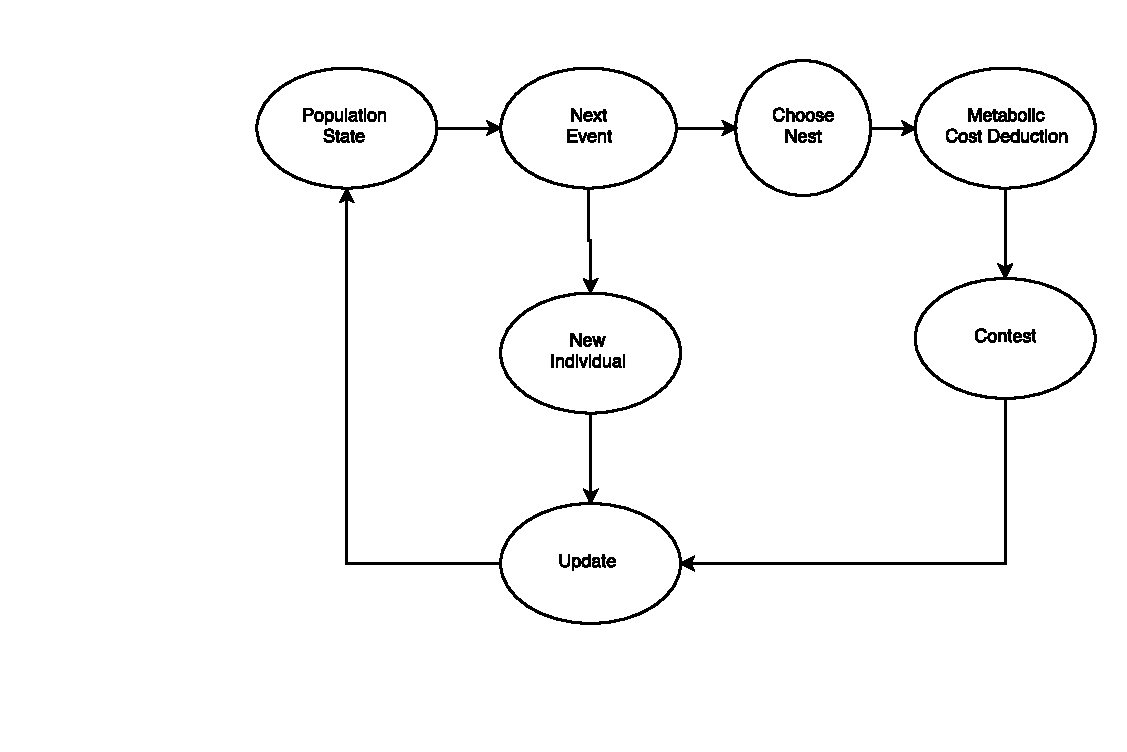
\includegraphics[width=15cm,height=15cm,keepaspectratio]{figures/event_algorithm}
\caption{Algorithm for modelling dynamics within the ``mature'' male population.}
\label{fig:events}
\end{figure}
\clearpage

\begin{figure}[h!]
\centering
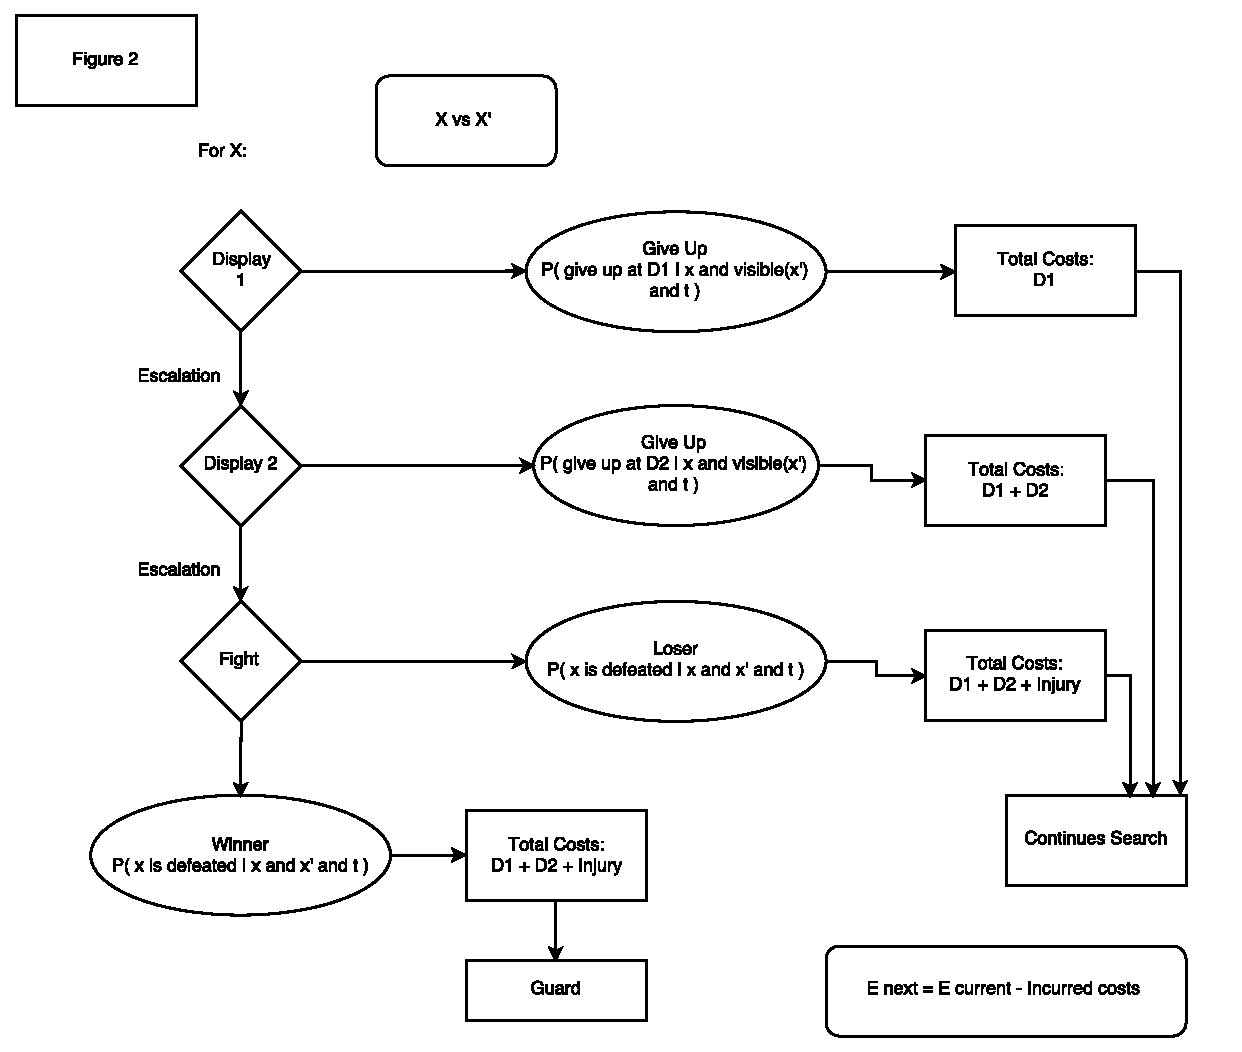
\includegraphics[width=15cm,height=15cm,keepaspectratio]{figures/contest_algorithm}
\caption{Algorithm for modelling contests behaviour within the ``mature'' male population.}
\label{fig:contests}
\end{figure}
\clearpage

\bibliography{refs}

\end{document}

